\documentclass[12pt]{article}
\usepackage{ctex}
\usepackage{listings}
\usepackage{xcolor}
\usepackage{hyperref}
\usepackage{graphicx}
\usepackage{float}
\usepackage{geometry}
\graphicspath{{imgs/}} % 图片文件夹的路径
\geometry{left=3cm,right=3cm,top=2cm,bottom=2cm}
\lstset{
	language=C++,
	basicstyle=\ttfamily,
	keywordstyle=\color{blue},
	commentstyle=\color{green!60!black},
	stringstyle=\color{orange},
	numbers=left,
	numberstyle=\tiny,
	frame=single,
	breaklines=true,
	linewidth=15cm 
}

\begin{document}
	\section{go语言死锁的讨论}
	\section{发送消息流程设计}
	\subsection{流程图}
	\subsection{引入了redis和不引入redis的对比}
	\subsection{使用tcp的效率}
	\subsection{使用udp的效率}
	\subsection{使用QUIC的效率}
	\section{将http协议升级为websocket协议}
	待补充
	\section{发送消息的设计和实现}
	需要:发送者ID,接收者ID,消息类型(文字、音频、图片等),消息的内容(说了什么话、发了什么图片),发送类型
	()
	
	\section{redis的引入}
	
	为什么需要引入redis:对于单机,使用websocket可以达到十万的并发。如果
	想要达到百万并发就需要引入redis了。
	\subsection{引入redis和不引入redis的对比}
	
	\section{token的引入}
	待实现(登陆需要引入token)
	\section{邮箱和手机号的校验}
	众所周知,邮箱应该是类似于xxx@hotmail.com的形式,手机号应该是186xxxxxxx这样的形式,因为在内存中我们采取的是用string来存储,因此在注册的时候,应该进行校验。在这里我们采用的是正则校验表达式。同时看到下图还有几个问题:
	\begin{enumerate}
		\item UID应该全为数字,类似于QQ号
		\item 密码和确认密码不应该明文出现,保护隐私
	\end{enumerate}
	
	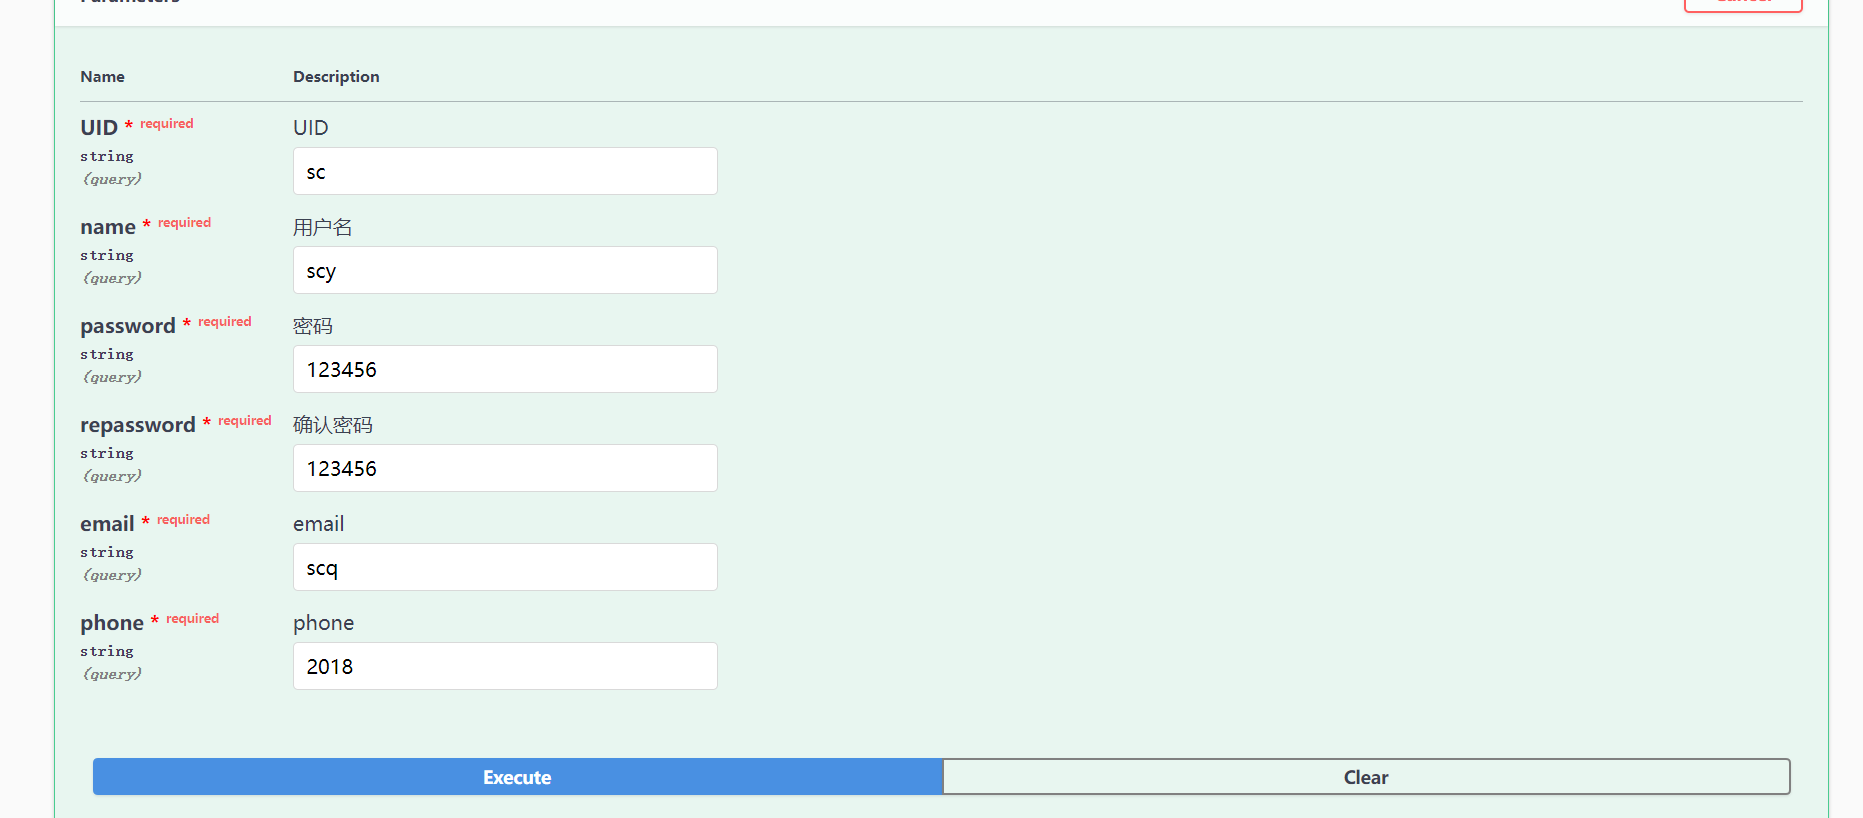
\includegraphics{16.png}
	
	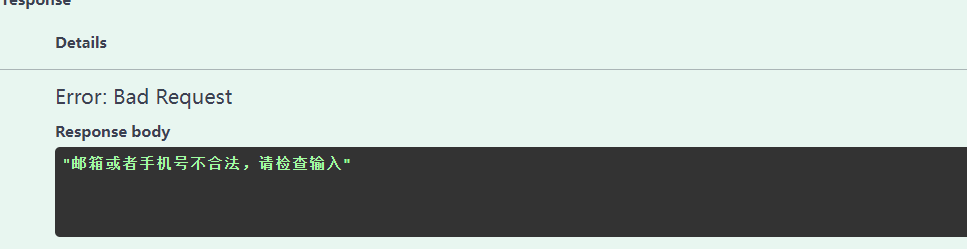
\includegraphics{17.png}
	
	正则表达式截图:
	
	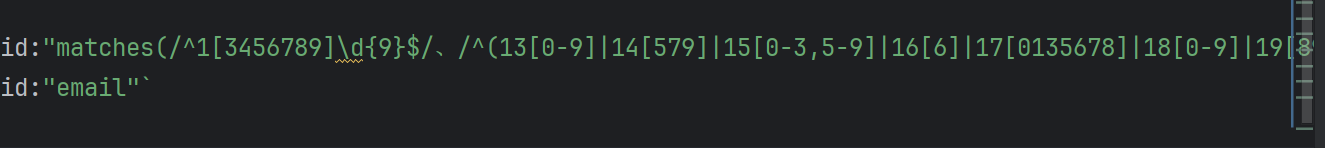
\includegraphics{18.png}
	
	\section{使用md5进行密码加密}
	为了解决什么问题:内部人员可能能看到账号密码/手机号,需要保护用户的隐私,同时也为了防止数据库被入侵,导致密码泄露。
	
	加密流程:随机数+用户的密码进行md5加密
	
	为什么需要引入随机数:防止彩虹表攻击,通常黑客会有一个表,比如123456对应e10adc3949ba59abbe56e057f20f883e。因此如果黑客能够看到数据库内的数据,可以对照彩虹表来得到原始密码。引入了随机数可以防止这种问题的发生,因为不知道随机数是多少。
	
	
	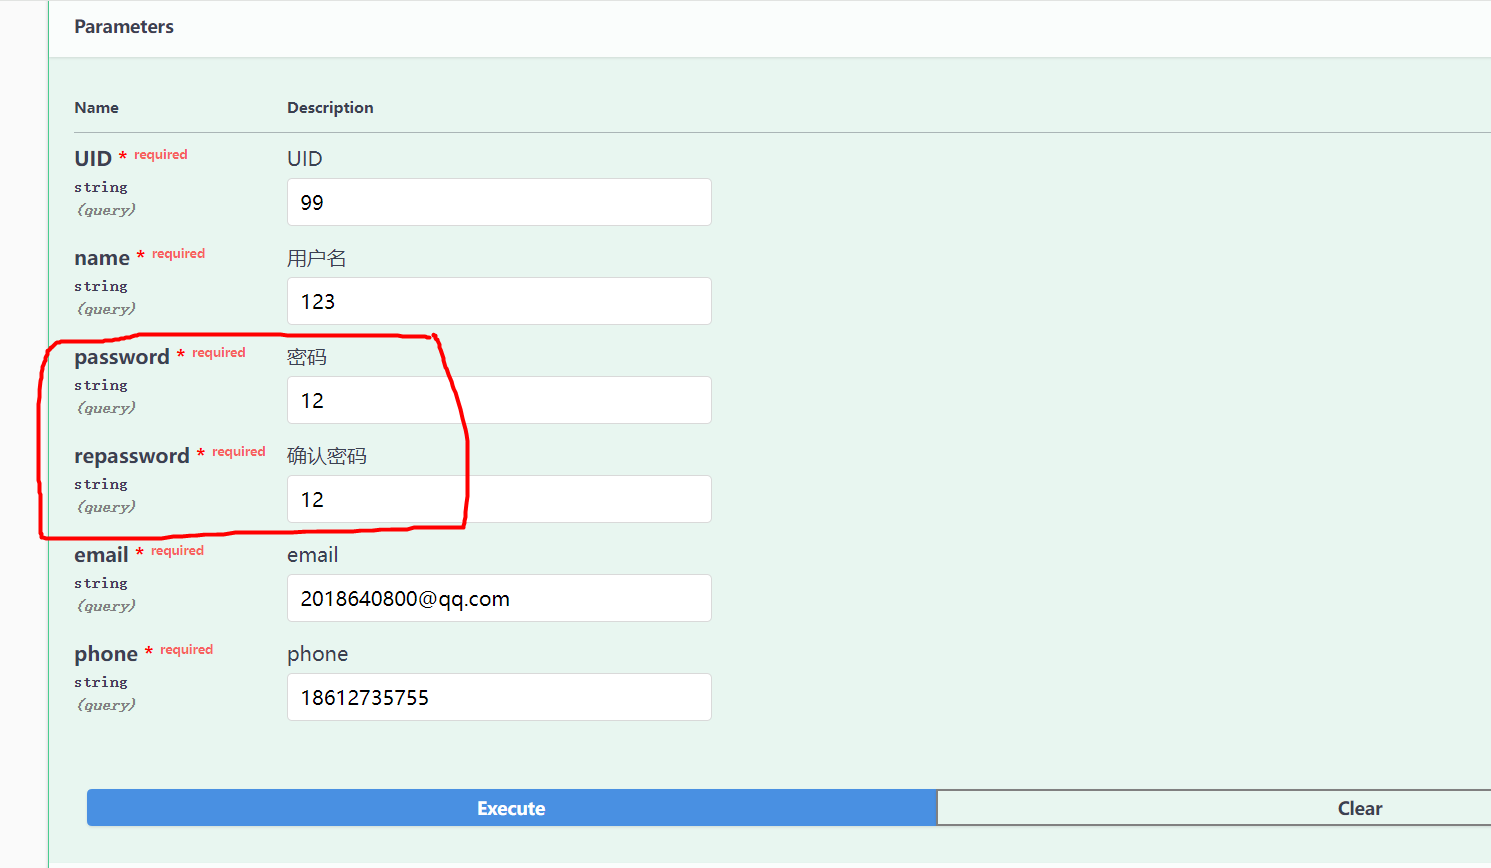
\includegraphics{19.png}
	
	加密后在数据库中的样子,可以看出是正确的:
	
	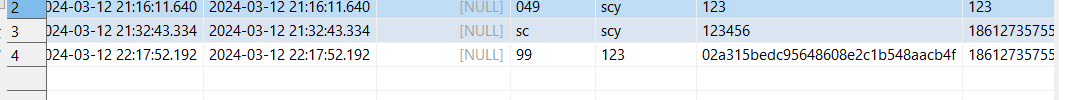
\includegraphics[scale=0.7]{20.png}
	
	
	
	\section{实现分布式唯一全局ID(雪花算法)}
	待更新
	
	\section{panic异常处理和数据库无法连接的问题的解决}
	有的时候程序会出现一些不符合我们预期的bug,这个时候我们需要捕获这个bug并且进行处理。如果不处理的话,线上服务可能会导致巨大的损失,且会导致后续难以排查问题。golang使用的是panic来解决这个问题。当发生panic的时候,报错如下:
	
	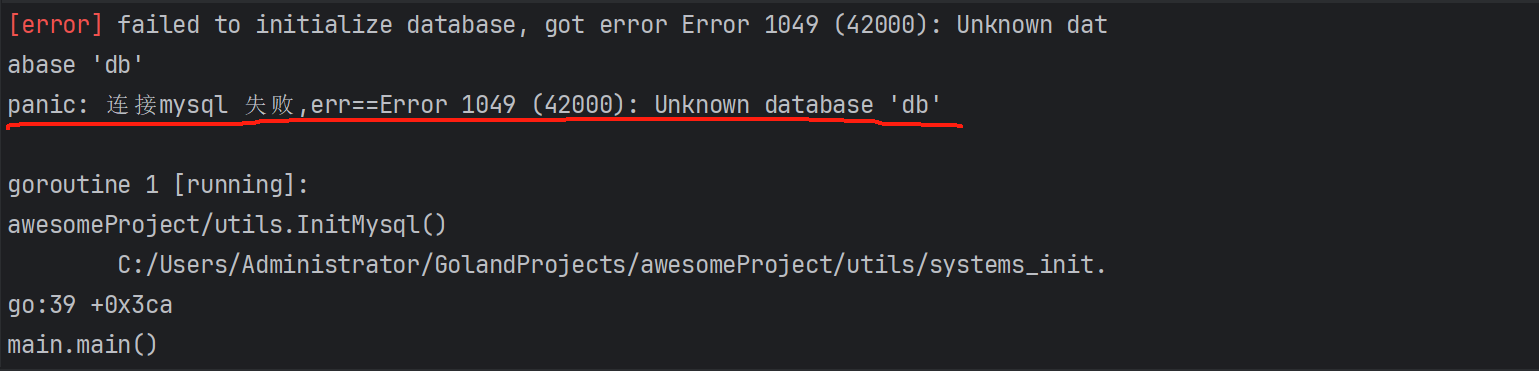
\includegraphics[scale=0.5]{3.png}
	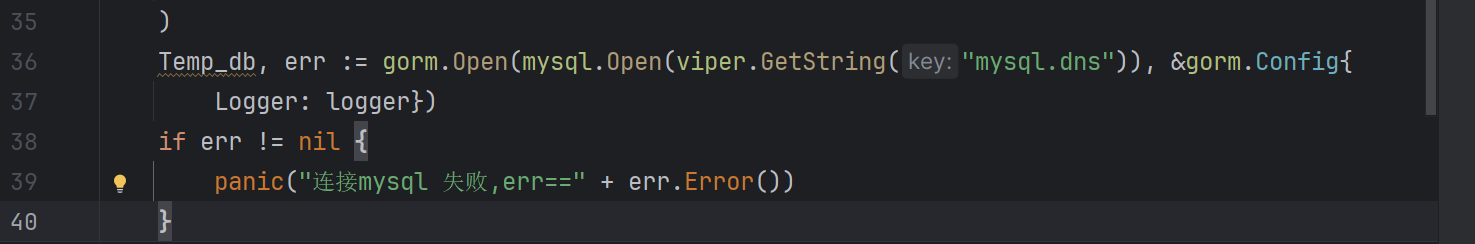
\includegraphics[scale=0.5]{4.png}
	经过排查发现是因为之前没有创建过这个数据库,使用mysql创建一个db,再进行连接就可以了:
	
	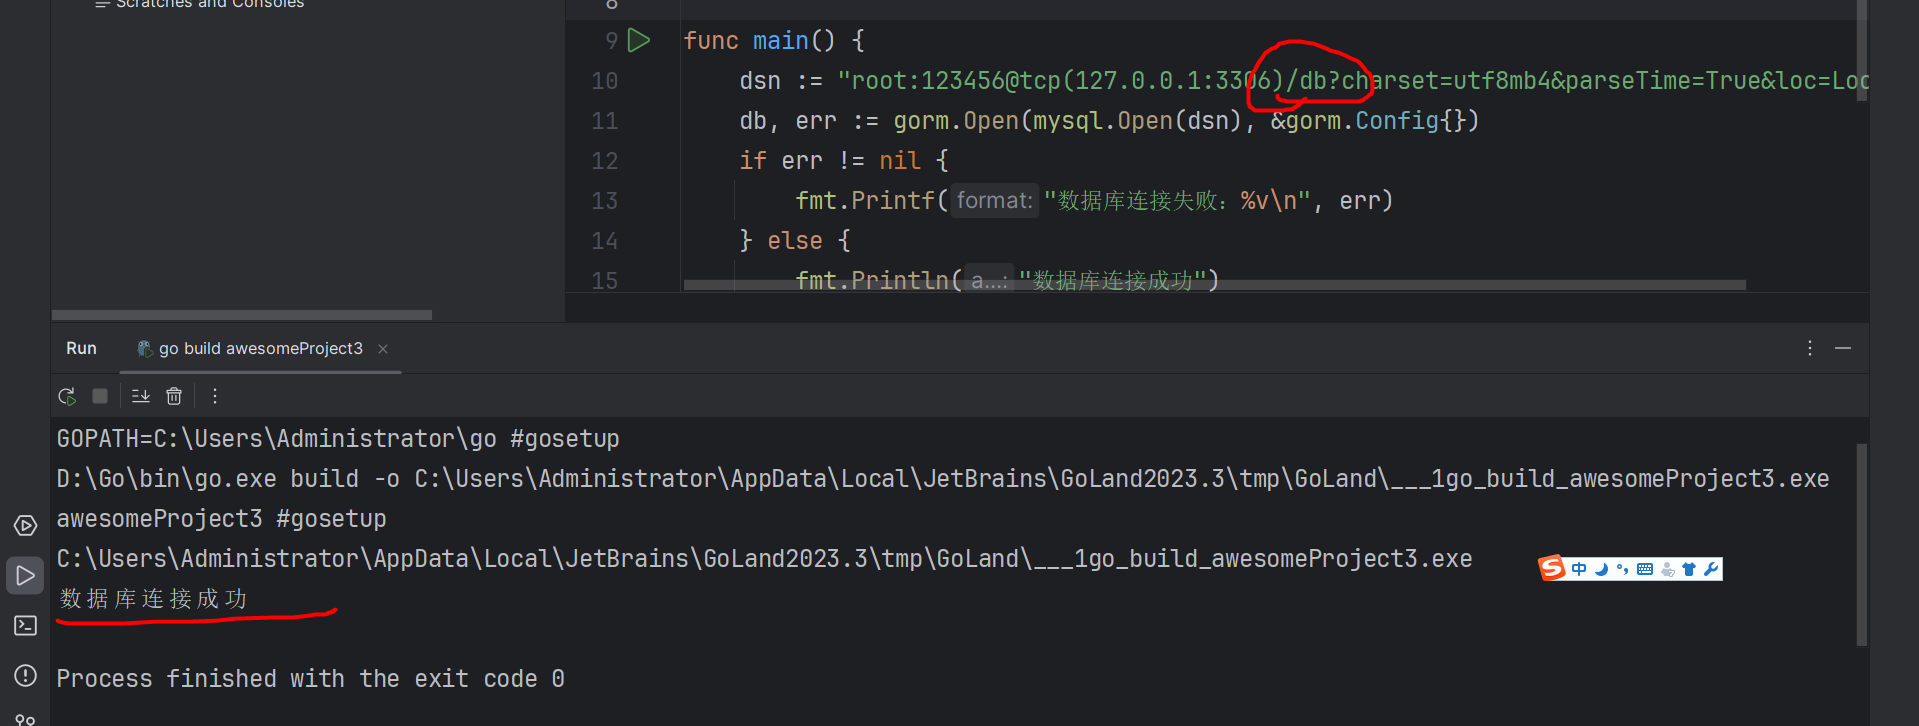
\includegraphics[scale=0.5]{5.png}
	
	\section{golang分层架构}
	问题引入:在创建用户的时候,报了循环引用的错误,具体的报错如下:
	
	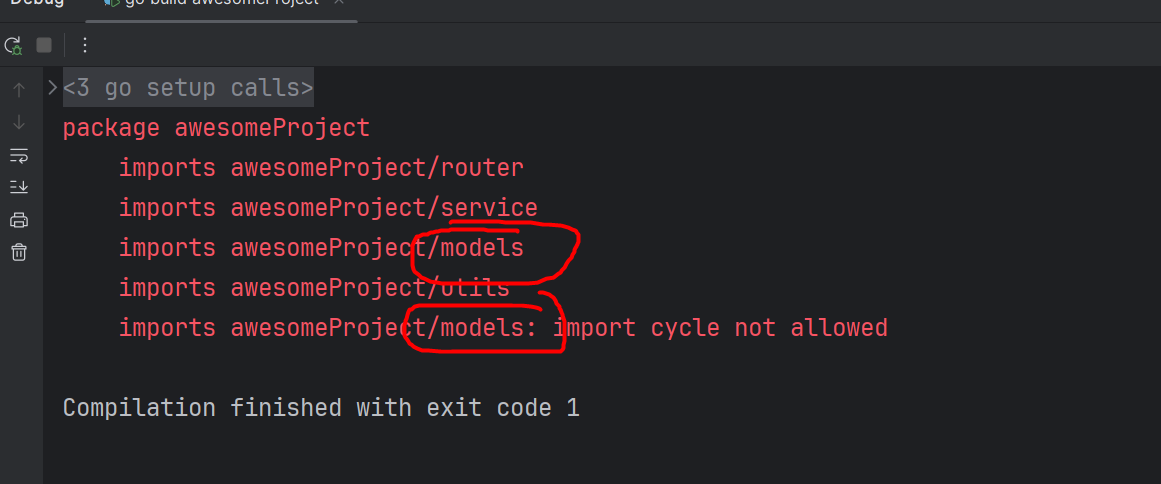
\includegraphics{6.png}
	
	问题解决:想起来在字节实习时候经常看到组里的代码是分层的,便去系统学习了一下golang的分层架构。
	
	一个比较贴近实际开发流程的分层架构如下:
	
	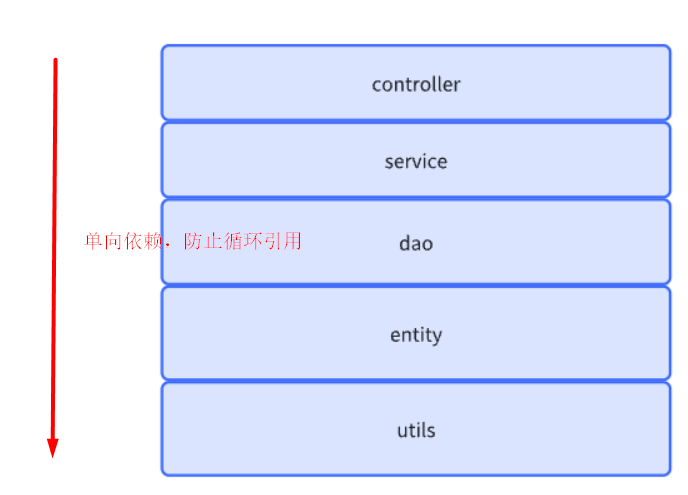
\includegraphics[scale=0.7]{7.png}
	
	\begin{enumerate}
		\item handlers: 处理器只做三件事情:接受请求解析入参、调用services完成业务逻辑、构造响应参数。handlers不包含业务代码逻辑,应该简单地作路由使用。
		\item services: 存放业务逻辑相关代码,是整个项目中逻辑最复杂的部分。
		\item dao:只进行对数据的CRUD,不含有业务逻辑。
		\item entity:entity包存放领域实体及其相关方法及枚举。只能提供最基本的和实体相关的方法,如定义了User结构体,提供IsValidUser方法判断该User是否有效等。
	\end{enumerate}
	
	在重新设计分层架构后,可以正常编译通过:
	
	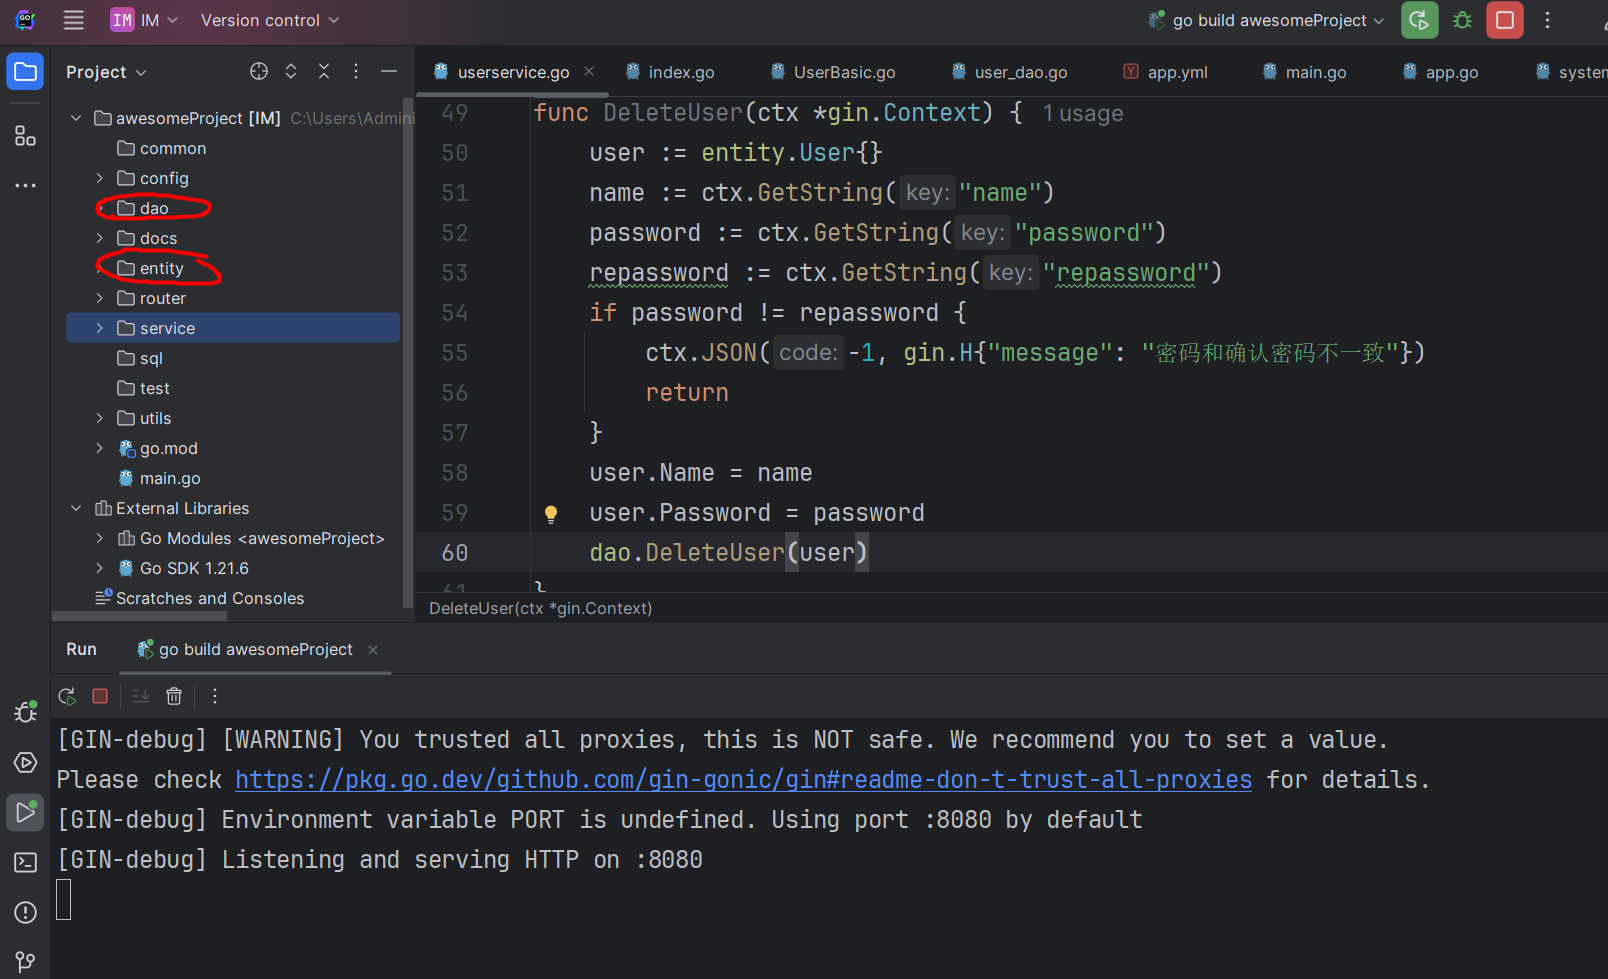
\includegraphics[scale=0.5]{8.png}
	
	\section{插入数据测试}
	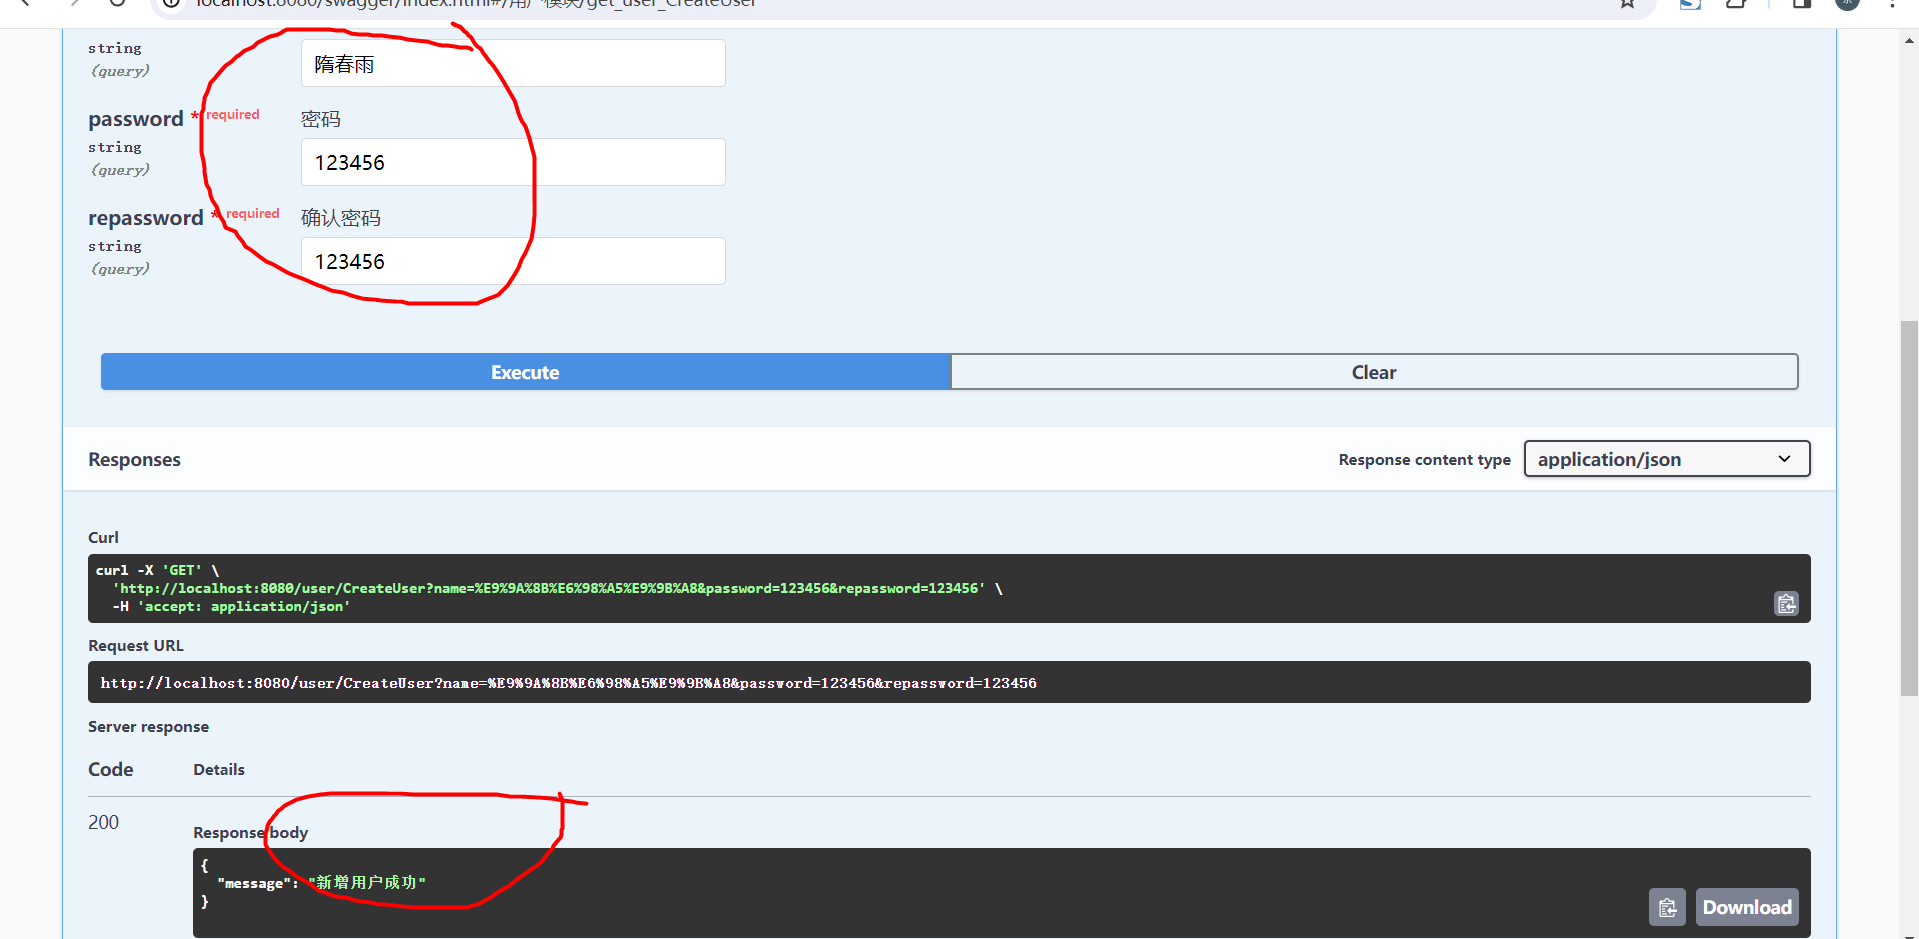
\includegraphics{9.png}
	可以看到是成功的插入到了数据库里边:
	
	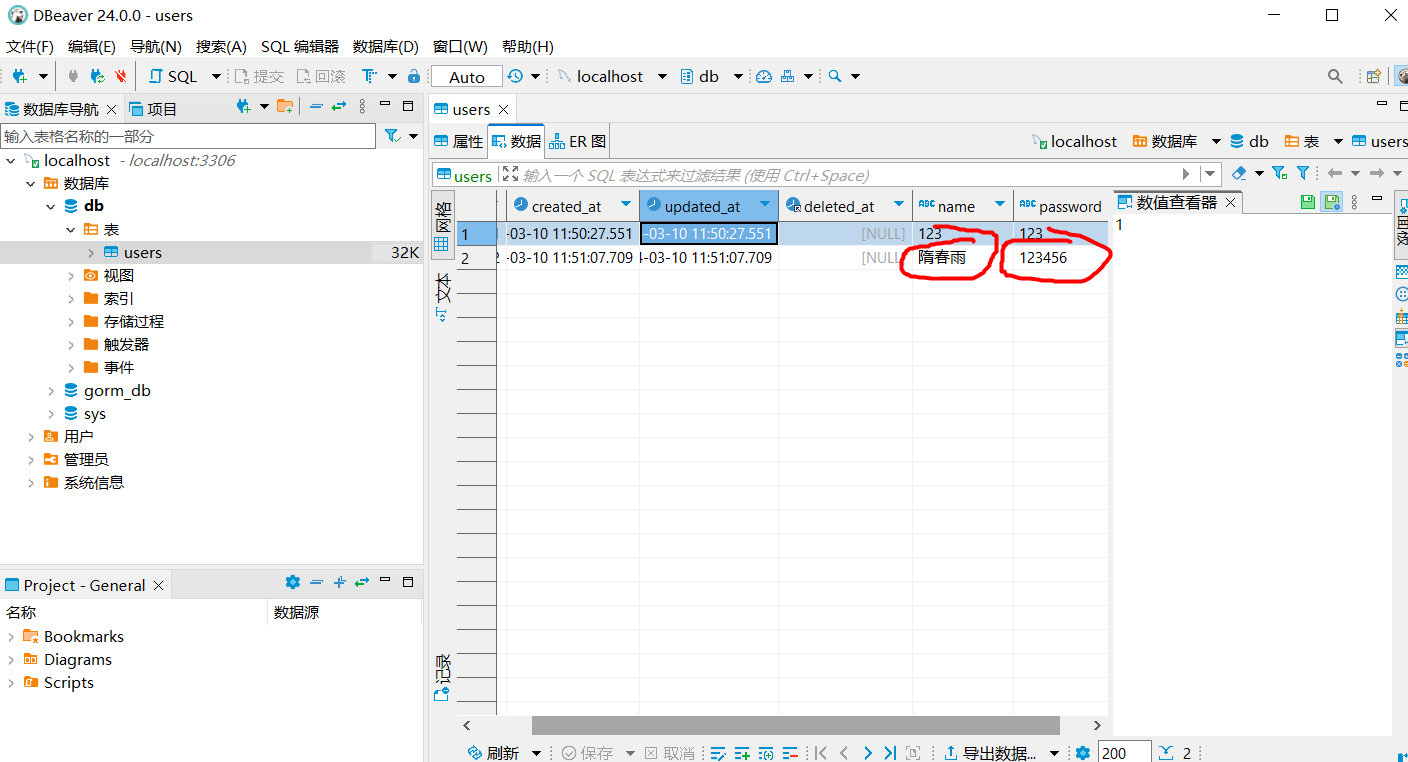
\includegraphics[scale=0.7]{10.png}
	\section{golang比较结构体的各个值是否相等}
	golang并不能够直接比较两个结构体是否相等(编译器没有实现),可以使用reflect.DeepEqual()函数来比较,如下图
	
	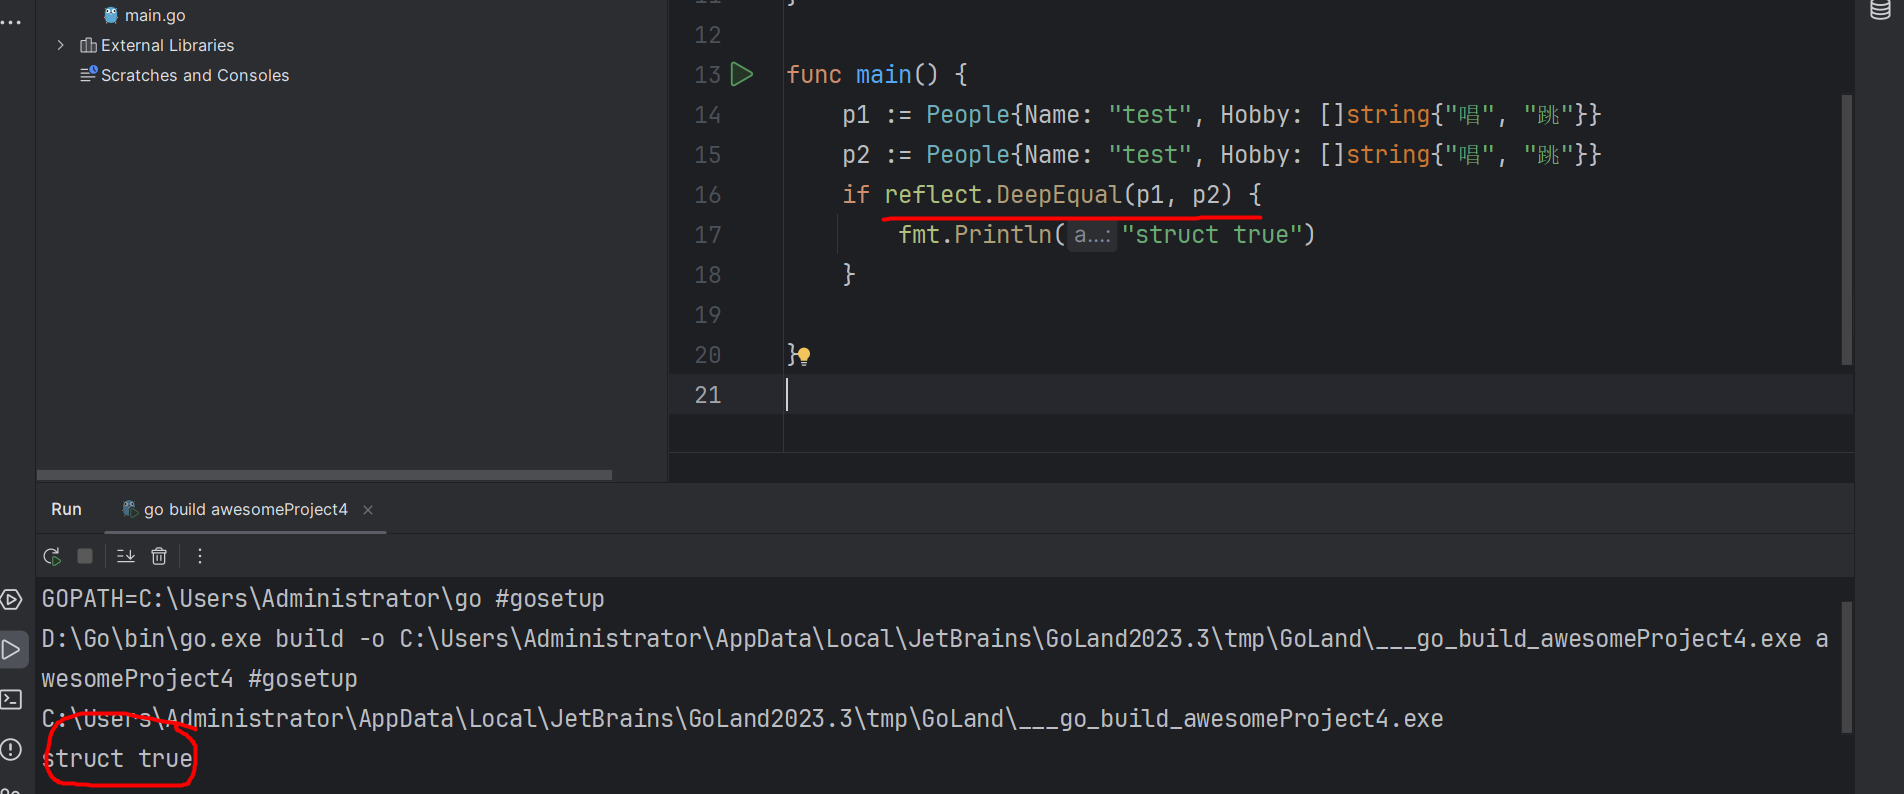
\includegraphics[scale=0.4]{11.png}
		
	\section{swagger}
	
	\subsection{问题背景}
	问题背景:之前也用过其他的API文档工具,但是最大的问题还是文档和代码是分离的。总是出现文档和代码不同步的情况。
	\subsection{为了解决什么问题}
	为了解决什么问题:自动化帮写接口说明文档。目前的项目基本都是前后端分离的项目,有时候后端更改完代码,有时候忘记更新了接口的说明文档
	\subsection{不同的Parameter Types的区别}
	Swagger 的 Parameter Types 可以分为以下几种:
	
	Path Parameters(路径参数):出现在 URL 路径中,通常用于标识资源。
	
	Query Parameters(查询参数):出现在 URL 查询字符串中,用于过滤或定位资源。
	
	Query Parameters更为常用,输入和输出如下:
	
	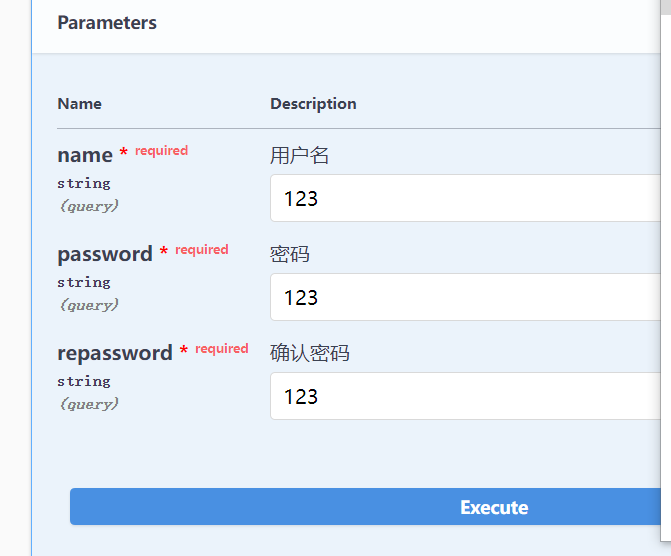
\includegraphics{1.png}
	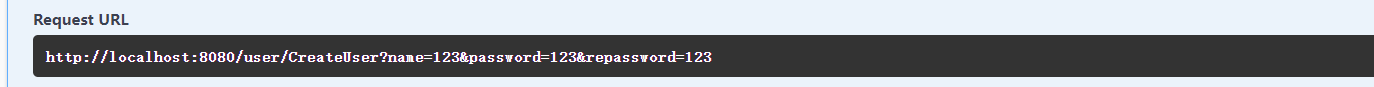
\includegraphics{2.png}
	
	Header Parameters(头部参数):出现在请求头部中,用于传递附加信息。
	
	Cookie Parameters(Cookie 参数):出现在 Cookie 头部中,用于在客户端和服务器之间传递状态信息。
	
	\section{HTTP状态码和swagger}
	\begin{itemize}
		\item 200: OK,请求成功,一般用于GET与POST请求。
		\item 301: Moved Permanently, 请求的资源已经被永久的移动到新的URL,返回信息包括一个新的URL。
		\item 304: Not modified, 未修改。查看本地缓存。
		\item 305: 使用代理。所请求的资源必须通过代理访问。
		\item 400: 客户端请求语法错误。
		\item 404: not found。
		\item 500:服务器内部错误。
	\end{itemize}
	
	\section{更新用户模块测试}
	输入数据:
	
	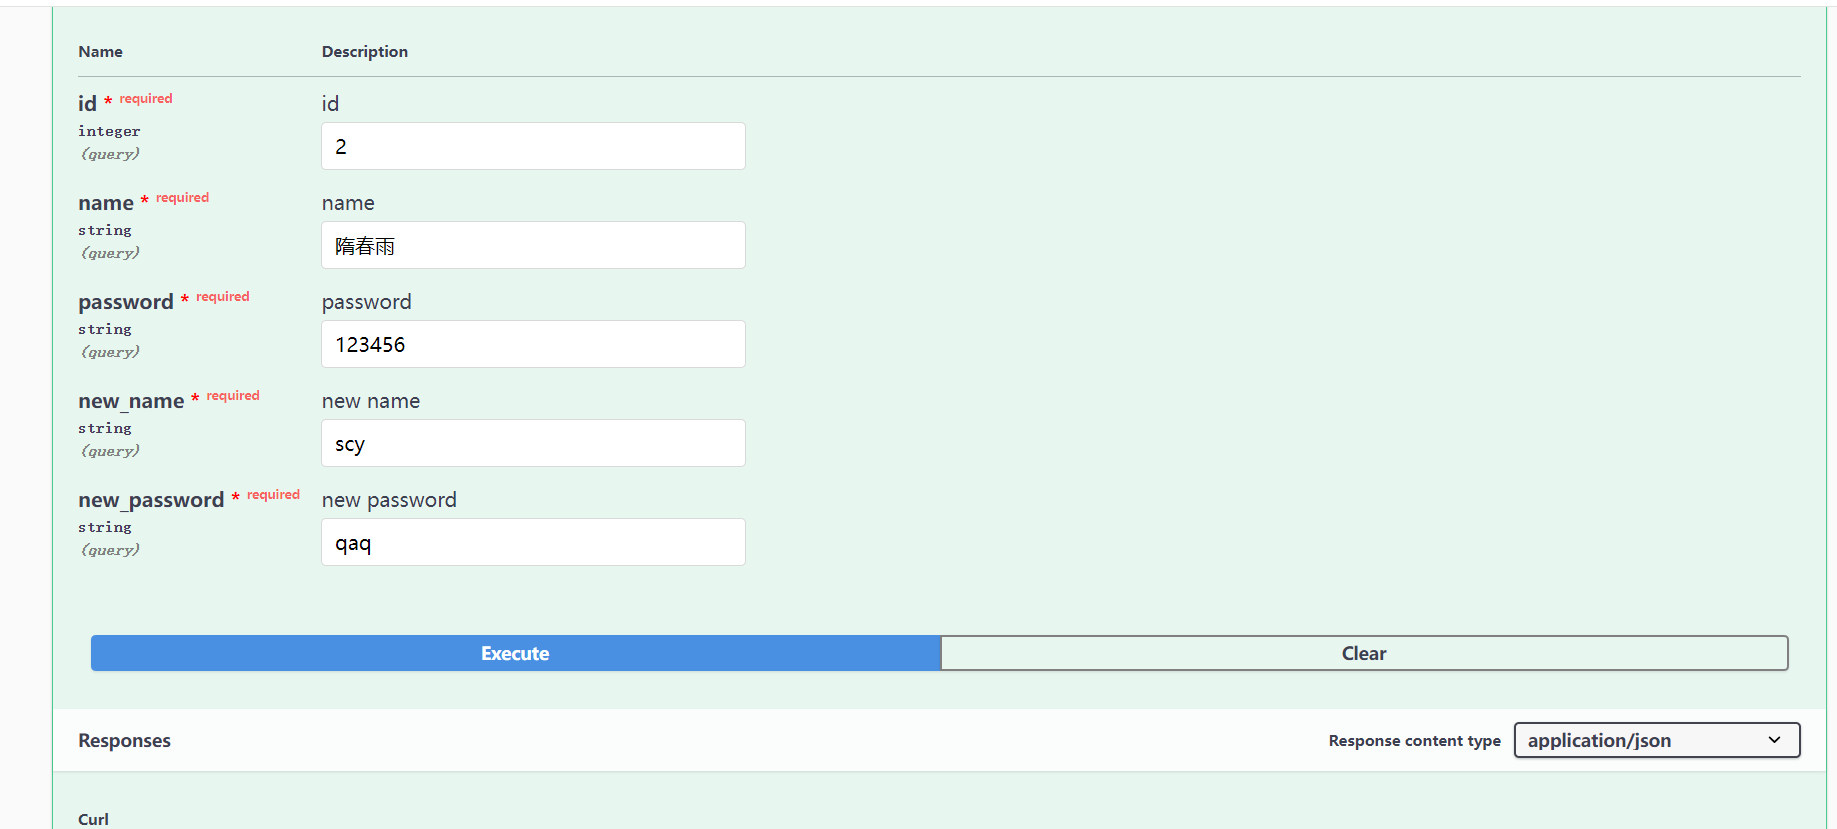
\includegraphics{12.png}
	
	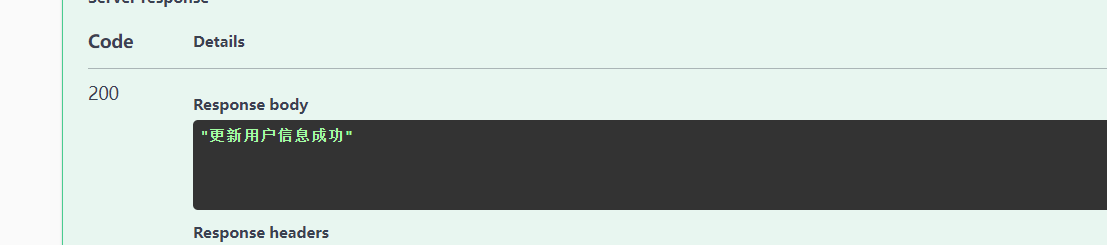
\includegraphics{13.png}
	
	db之前的数据:
	
	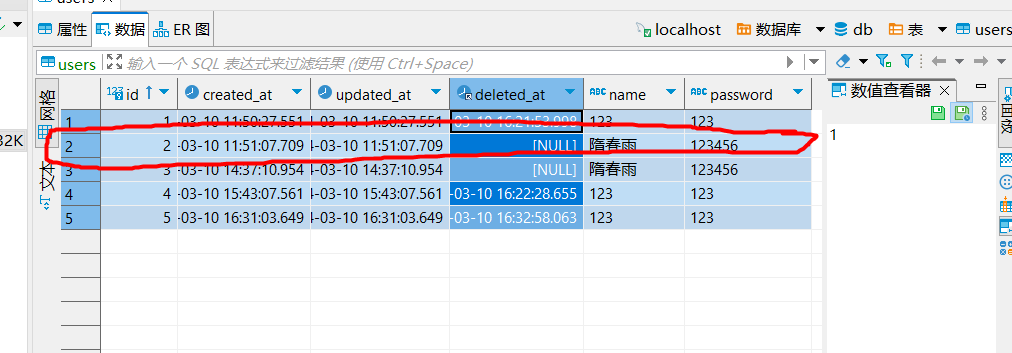
\includegraphics{14.png}
	
	更新之后的数据:
	
	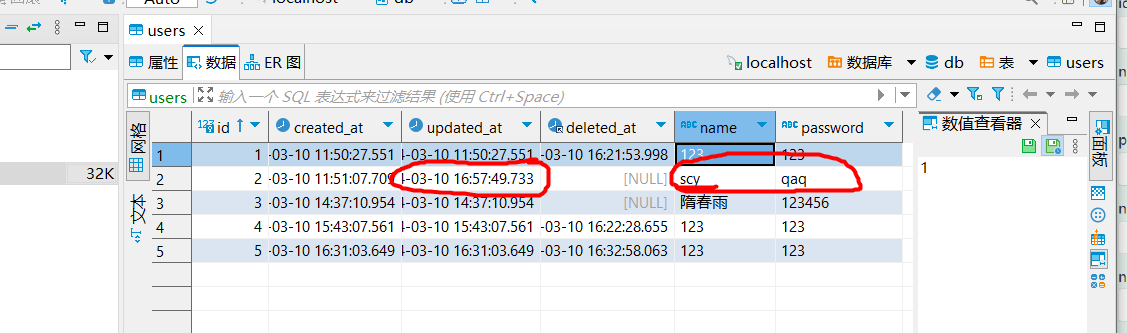
\includegraphics{15.png}
	
	可以看出来,更新成功
	
\end{document}







